\section{Tổng quan về tái tạo mô hình mây điểm 3D từ ảnh 2D}
\label{sec:tong_quan_3d}
Trong lĩnh vực xử lý ảnh và thị giác máy tính, bài toán dựng 3D từ ảnh 2D đã và đang trở thành một hướng nghiên cứu quan trọng, với các ứng dụng thực tiễn như dựng mô hình kiến trúc, khảo sát địa hình, và khảo sát các đối tượng kỹ thuật phức tạp như trạm thu phát sóng di động. Quá trình dựng 3D từ ảnh 2D thường được chia thành các giai đoạn chính được mô tả trong Hình \ref{fig:3D_pipeline}, bao gồm: (1) thu thập và tiền xử lý dữ liệu ảnh, (2) trích xuất đặc trưng và khớp nối ảnh, (3) xây dựng đám mây điểm 3D, (4) tái tạo lưới bề mặt, và (5) tạo kết cấu để hoàn thiện mô hình 3D. Trong đó, việc xây dựng đám mây điểm 3D đóng vai trò trung tâm, là bước nền tảng và cũng là bước quan trọng nhất để chuyển từ dữ liệu ảnh 2D sang không gian 3D, cung cấp thông tin về cấu trúc không gian của đối tượng.

\begin{figure}[H]
    \centering
    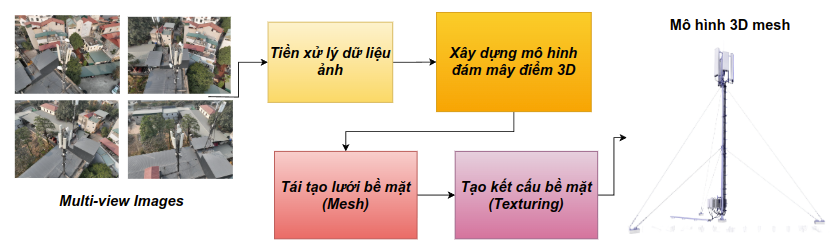
\includegraphics[width=\linewidth]{figures/c2/quy_trinh_3d_from_image.png}
    \caption{Quy trình xây dựng mô hình 3D hoàn chỉnh từ ảnh chụp 2D đa góc nhìn.}
    \label{fig:3D_pipeline}
\end{figure}

Trong phạm vi nghiên cứu của luận văn, luận văn tập trung giải quyết bài toán tái dựng đám mây điểm 3D chi tiết, chính xác cho đối tượng cột ăng-ten. Đám mây điểm 3D không chỉ cung cấp thông tin về hình dạng tổng thể của cột ăng-ten mà còn hỗ trợ phân tích thông tin kĩ thuật kết cấu của cột, cũng như hỗ trợ nhận diện, kiểm đếm, đo đạc các thông số kỹ thuật của các thiết bị được lắp đặt trên cột. Đặc biệt, trong các ứng dụng thực tiễn, đám mây điểm 3D cũng có thể được sử dụng để kiểm tra độ chính xác của thiết kế, phát hiện hư hỏng, hoặc lập kế hoạch bảo trì mà không nhất thiết phải dựng mô hình 3D hoàn chỉnh. Tuy nhiên, do cột BTS thường có cấu trúc phức tạp, bề mặt thiết bị trơn nhẵn, đồng màu nên việc tạo đám mây điểm 3D chi tiết, chính xác cho cột viễn thông là một thách thức lớn.

\subsection{Giới thiệu bài toán tái tạo mô hình đám mây điểm 3D từ ảnh 2D}
\label{subsec:gioi_thieu_bai_toan}
Tái tạo mô hình đám mây điểm 3D từ các hình ảnh 2D là một trong những lĩnh vực nghiên cứu nền tảng và có lịch sử lâu đời trong cả thị giác máy tính và quang trắc học. Đám mây điểm 3D là tập hợp các điểm trong không gian ba chiều, mỗi điểm được xác định bởi tọa độ $(x, y, z)$ và có thể kèm theo thông tin bổ sung như màu sắc. Đầu vào của bài toán là một tập các ảnh 2D đảm bảo một tỉ lệ chồng lấp nhất định giữa các ảnh liền kề nhau trong quỹ đạo chụp. Đầu ra mong muốn là một biểu diễn đám mây điểm 3D của cảnh, phổ biến nhất là dưới dạng một đám mây điểm dày đặc, chi tiết. Quá trình tái tạo đám mây điểm 3D từ ảnh 2D là một bài toán đối mặt với nhiều thách thức. Các thuật toán cần phải đủ mạnh mẽ để đối phó với sự thay đổi về điều kiện chiếu sáng, góc nhìn, sự che khuất, các vùng bề mặt không có hoặc ít đặc trưng thị giác, và các cấu trúc có tính chất lặp lại - những yếu tố thường gặp khi chụp ảnh các cấu trúc công nghiệp như cột ăng-ten viễn thông.

\subsection{Các hướng tiếp cận chính}
\label{subsec:huong_tiep_can}
Trong lĩnh vực thị giác máy tính và quang trắc học, có nhiều phương pháp khác nhau để giải quyết bài toán tái tạo 3D. Luận văn này tập trung vào các phương pháp chỉ sử dụng ảnh 2D thu được từ máy ảnh. Hiện nay, có hai hướng tiếp cận chính, phổ biến trong lĩnh vực này: phương pháp truyền thống dựa trên hình học và phương pháp hiện đại dựa trên Học sâu.

\textbf{Phương pháp truyền thống dựa trên hình học:} Đây là hướng tiếp cận đã được phát triển và hoàn thiện trong nhiều thập kỷ, thường bao gồm hai giai đoạn chính:
\begin{itemize}
    \item Phục dựng cấu trúc từ chuyển động: Giai đoạn này tập trung vào việc ước lượng đồng thời các tham số nội tại, camera pose cho từng ảnh chụp, cũng như cấu trúc hình học của cảnh dưới dạng một tập hợp các điểm 3D thưa thớt. Nền tảng của SfM dựa trên việc phát hiện, mô tả và khớp nối các điểm đặc trưng giữa các ảnh, sau đó sử dụng các ràng buộc hình học đa góc nhìn và tối ưu hóa để đạt được kết quả chính xác \cite{Schonberger16SFMRevisited}. 
    \item Tái tạo lập thể đa góc nhìn: Sau khi đã có được camera pose và cấu trúc thưa từ SfM, MVS được sử dụng để tái tạo cấu trúc hình học dày đặc bằng cách ước định độ sâu cho các điểm ảnh trong ảnh dựa trên nguyên tắc tối ưu hóa sự tương đồng quang học giữa điểm ảnh được xét và hình chiếu của điểm 3D tương ứng với độ sâu của điểm ảnh đó khi chiếu lên các bức ảnh ở góc nhìn khác nhau\cite{Seitz2006comparison, Furukawa2015multi}. Kết quả của MVS thường là một đám mây điểm dày đặc hoặc một lưới 3D.
\end{itemize}
Phương pháp SfM kết hợp với MVS này đã chứng minh được sự hiệu quả và độ tin cậy cao, đặc biệt với các cảnh có đặc trưng bề mặt đối tượng và điều kiện chụp ảnh tốt. Các công cụ mã nguồn mở mạnh mẽ như COLMAP, OpenMVS là các công cụ phổ biến, được sử dụng rộng rãi trong cộng đồng nghiên cứu khoa học.

\textbf{Phương pháp hiện đại dựa trên Học sâu}: Sự bùng nổ của các kiến trúc mạng học sâu đã mang lại những thay đổi và cải tiến đáng kể cho bài toán tái tạo đám mây điểm 3D:
\begin{itemize}
    \item Cải thiện phương pháp truyền thống: Học sâu được ứng dụng kết hợp hoặc thay thế cho các bước của phương pháp SfM kết hợp với MVS để nâng cao hiệu năng. Các bộ phát hiện và mô tả đặc trưng dựa trên học sâu như SuperPoint \cite{detone2018superpoint}, DISK \cite{tyszkiewicz2020disk} và các bộ khớp nối đăc trưng mạnh mẽ như SuperGlue \cite{sarlin2020superglue}, LightGlue \cite{lindenberger2023LightGlue} có thể hoạt động hiệu quả hơn các phương pháp truyền thống trong các điều kiện khó khăn như thay đổi ánh sáng, đặc trưng bề mặt đối tượng ít,... Các kỹ thuật dựa trên học sâu cũng được áp dụng để cải thiện các bước trong MVS như các mô hình MVSNet \cite{Yao2018mvsnet}, SAFE-MVS \cite{wei2023safemvs} với mục tiêu giải quyết các nhược điểm của MVS như thời gian tính toán lâu, kém chi tiết khi tái tạo mây điểm cho các bề mặt đối tượng ít đặc trưng.
    \item Biểu diễn ngầm và kết xuất nơ-ron: Một hướng tiếp cận hoàn toàn mới và đột phá là sử dụng mạng nơ-ron để học một biểu diễn 3D ngầm của cảnh trực tiếp từ ảnh 2D và camera pose. Mô hình NeRF \cite{Mildenhall2020NeRF} là phương pháp tiêu biểu nhất cho hướng này. NeRF học một mạng nơ-ron nhằm biểu diễn cho một không gian 3D liên tục, trong đó, ánh xạ mỗi tọa độ 3D và hướng nhìn tại điểm đó vào một trường màu sắc và mật độ. NeRF cho phép kết xuất các ảnh mới từ các góc nhìn tùy ý với chất lượng rất cao. Mặc dù mục tiêu ban đầu của NeRF là kết xuất hình ảnh góc nhìn mới, các phương pháp trích xuất thông tin hình học từ biểu diễn NeRF cũng đang được phát triển mạnh mẽ cho phép NeRF có thể tái tạo một đám mây điểm 3D cho độ chi tiết, chất lượng rất cao. NeRF và các biến thể của nó đặc biệt mạnh trong việc xử lý các hiệu ứng phụ thuộc góc nhìn và các bề mặt phức tạp, ít đặc trưng.
\end{itemize}

Luận văn sẽ đi sâu vào tìm hiểu các thành phần cốt lõi của các thuật toán trong cả phương pháp truyền thống và hiện đại là SfM, MVS và NeRF trong các mục tiếp theo.